\documentclass[11pt,letterpaper]{article}

% Load some basic packages that are useful to have
% and that should be part of any LaTeX installation.
%
% be able to include figures
\usepackage{graphicx}
% get nice colors
\usepackage{xcolor}

% change default font to Palatino (looks nicer!)
\usepackage{apjfonts}
% load some useful math symbols/fonts
\usepackage{latexsym,amsfonts,amsmath,amssymb}

% comfort package to easily set margins
\usepackage[top=1in, bottom=1in, left=1in, right=1in]{geometry}

% control some spacings
%
% spacing after a paragraph
\setlength{\parskip}{.15cm}
% indentation at the top of a new paragraph
\setlength{\parindent}{0.0cm}


\begin{document}

\begin{center}
\Large
{\bf Ay190 -- Worksheet 6} \\
\large
Xiangcheng Ma \\
Date: \today
\end{center}

\section*{Discrete Fourier Transform}

(a) The function {\tt dft(x)}  that computes discrete Fourier transform is achieved in module ``{\tt dft.py}". To test this function, I uniformly generate 30 point in $[-2,2]$ for a Gaussian function
\begin{equation}
  f(x) = \frac{1}{\sqrt{2\pi}} e^{-\frac{x^2}{2}} ,
\end{equation}
and calculate the discrete Fourier transform using my function and the {\tt np.fft.fft} function. The results are listed in Table~\ref{tb}. Their results are consistent within my output accuracy, i.e., $10^{-9}$.
\begin{table}[h]
\centering
\begin{tabular}{ccccc}
\hline\hline
$t$ (days) & E & $x$ (AU) & $y$ (AU) & steps \\
\hline
\multicolumn{5}{c}{$e=0.0167$} \\
\hline
91.0 & 1.58209228899 & -0.0112957219731 & 0.999796755471 & 4 \\
182.0 & 3.13096420068 & -0.999943518526 & 0.0106267706437 & 2 \\
273.0 & 4.67948910053 & -0.0328939450239 & -0.99931946851 & 4 \\
\hline
\multicolumn{5}{c}{$e=0.99999$} \\
\hline
91.0 & 2.30664638749 & -0.671217514443 & 0.00331500920351 & 7 \\
182.0 & 3.13618964107 & -0.999985403763 & 2.41628286027e-05 & 3 \\
273.0 & 3.96364377765 & -0.680720102446 & -0.00327602643159 & 7 \\
\hline\hline
\end{tabular}
\label{table}
\caption{Kepler Motion}
\end{table}


(b) For 100 calculations, the accumulated time versus $N^2$ are plotted in Figure~\ref{fig1}. It shows basically a linear relation.
\begin{figure}[bth]
\centering
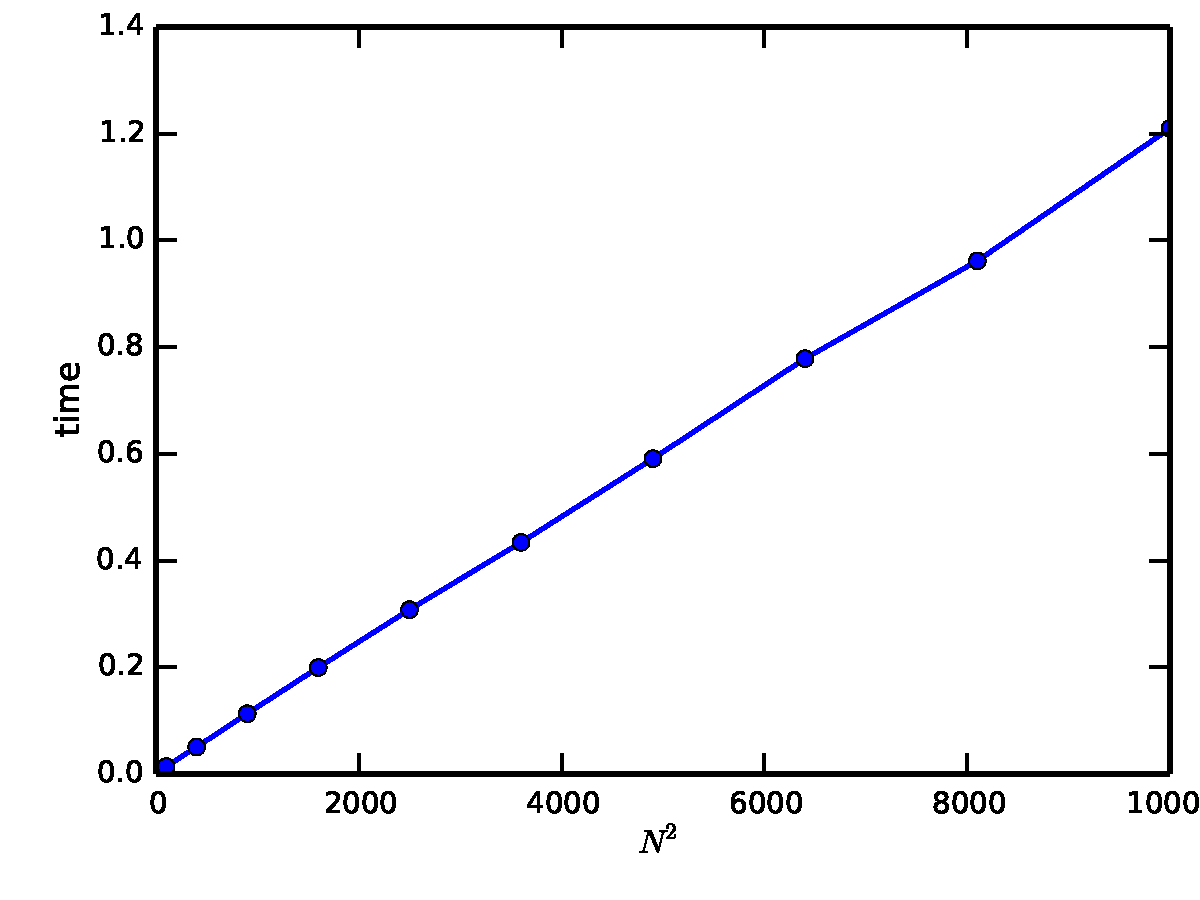
\includegraphics[width=0.9\textwidth]{fig1.pdf}
\caption{Computer time for {\tt dft(x)} function.}
\label{fig1}
\end{figure}

(c) For 100 calculations, the accumulated time versus $N\log(N)$ are plotted in Figure~\ref{fig2}. Although some scatter exists, the relation is in general linear.
\begin{figure}[bth]
\centering
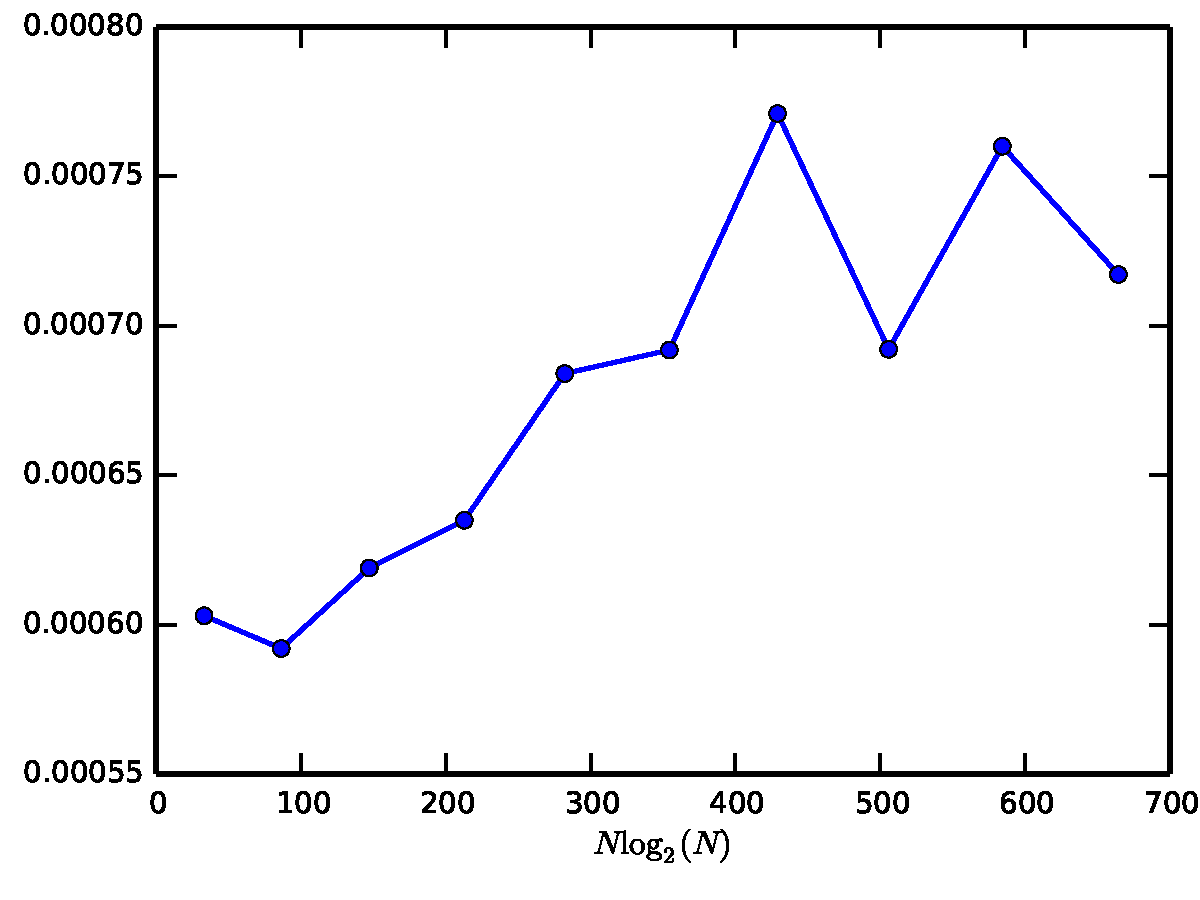
\includegraphics[width=0.9\textwidth]{fig2.pdf}
\caption{Computer time for {\tt dft(x)} function.}
\label{fig2}
\end{figure}

\end{document}
